\chapter{Risultati dell'analisi linguistica}

\section{Informazioni linguistiche di base}
Dopo aver compreso la natura dei nostri dati e aver eliminato valori nulli o non utili, concentrandosi sui tweet e analizzando i loro aspetti linguistici cercando di estrarre informazioni utili, utilizzando la libreria NLTK - Natural Language ToolKit\footnote{http://www.nltk.org}


% Prima di poter effettuare queste operazioni è stato necessario ripulire i tweet da eventuali elementi (spazi doppi, punteggiatura, lettere maiuscole, links ecc.) e simboli non utili ("@" e "\#" che precedono le menzioni e gli hashtag) , utilizzando le \textbr{espressioni regolari/Regular expression} e dalle cosiddette \textit{stopwords}, ossia tutte quelle parole che pur essendo molto comuni all'interno della lingua non sono funzionali al fine delle analisi linguistiche e non vengono indicizzate dai motori di ricerca (es. articoli, congiunzioni, preposizioni, ecc.)\\

Ciascun tweet è stato poi diviso in \textbf{tokens}, i quali sono stati successivamente \textit{lemmatizzati}, ossia riportati alla loro forma originaria \\
I token totali estratti dal corpus sono 146921 e in media ciascun tweet contiene circa 15 tokens (figura \ref{lunghezza_tok_tweet}); per quanto riguarda invece la lunghezza media dei tweet, ossia da quante lettere è composto ciascun token, la maggior parte dei token ha una lunghezza di 10 lettere (Figura \ref{Lunghezza_tok})

\begin{figure}[H]
	\centering
	\subfloat[]
	{
		\label{lunghezza_tok_tweet}
		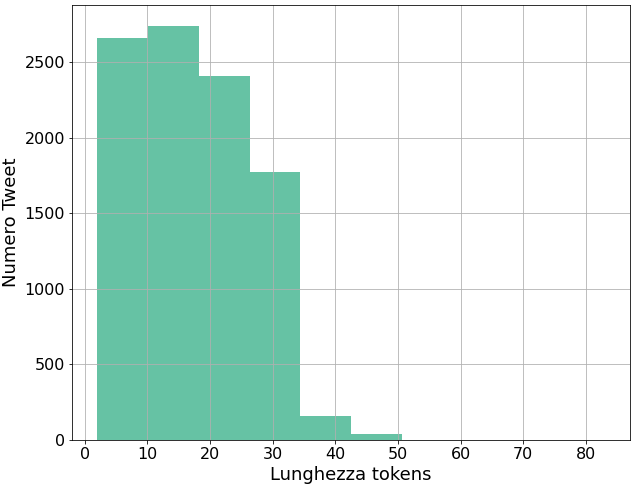
\includegraphics[width=.46\textwidth]{img/lunghezza_media_tokens_unici.png}
	}
	\quad
	\subfloat[]
	{
		\label{Lunghezza_tok}
		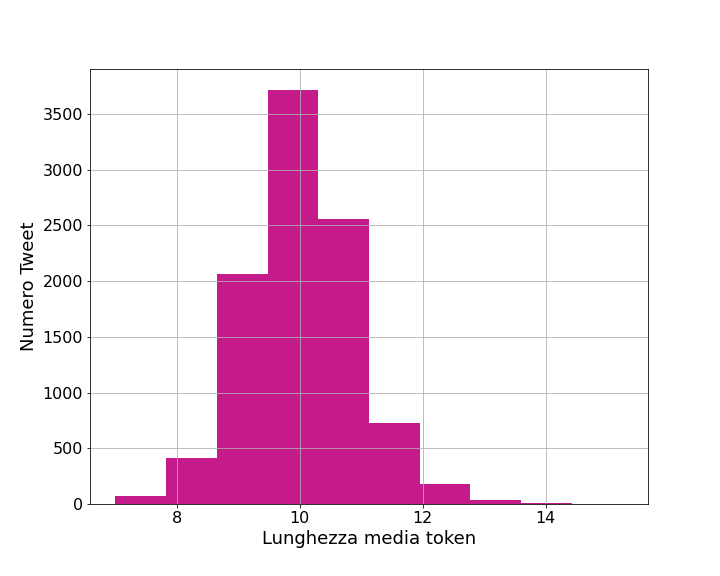
\includegraphics[width=.46\textwidth]{img/lunghezza_media_tokens.png}
	}    
	\setlength{\belowcaptionskip}{-10pt}
	\caption{Quantità media di tokens contenuti in ciascun tweet e lunghezza media dei tokens}
	\label{fig: tokens}
\end{figure}

\section{Analisi delle parole più frequenti}
Successivamente, si è provveduto ad analizzare quali fossero le parole più frequenti all'interno dei tweet, calcolando per ciascuna la propria frequenza all'interno del corpus.
\begin{figure} [H]
    \centering
    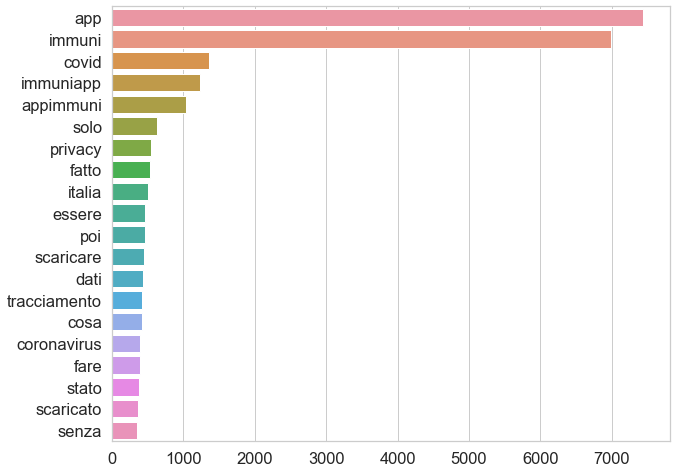
\includegraphics[width = 0.8\textwidth]{img/freq_toj.jpg}
    \caption{20 parole più utilizzate dagli utenti per discutere del tema App Immuni}
    \label{fig:most_common_20_tok}
\end{figure}
Analizzando le 20 parole più utilizzate all'interno dei tweet (figura \ref{fig:most_common_20_tok}), è possibile notare come tutte siano collegate al tema App Immuni e in generale al macro tema Coronavirus. Oltre a queste, altre due parole molto utilizzate sono \textit{dati}, che compare 436 volte nei tweet, e \textit{privacy} che compare 548 volte. Queste due parole sono molto importanti nella discussione sul tema App Immuni, in quanto spesso gli utenti sono molto restii a cedere i propri dati, soprattutto di natura sanitaria o di geo localizzazione, ad una applicazione di proprietà istituzionale, nonostante questi vengono ceduti ad altre piattaforme come ad esempio quelle dei maggiori \textit{social networks.}


Questa reticenza nella cessione dei dati è forse sintomo di una scarsa informazione da parte degli organi istituzionali, un fenomeno che ha poi portato al calo dei download di Immuni e al suo progressivo inutilizzo.


\section{Analisi degli \textit{hashtag} utilizzati}
Un altro aspetto che si è scelto di analizzare in questa fase del lavoro sono gli \textbf{hashtag} utilizzati dagli utenti per esprimersi sul tema App Immuni.
Gli hashtag sono uno strumento molto utilizzato su Twitter in quanto permettono di raggruppare tutti i tweet scritti su un particolare tema, facilitando all'utente la loro reperibilità; è sufficiente, infatti, che l'utente clicchi su quel particolare hashtag per risalire a tutti i tweet scritti sul tema.
% analisi hashtag
\begin{figure} [H]
    \centering
    
    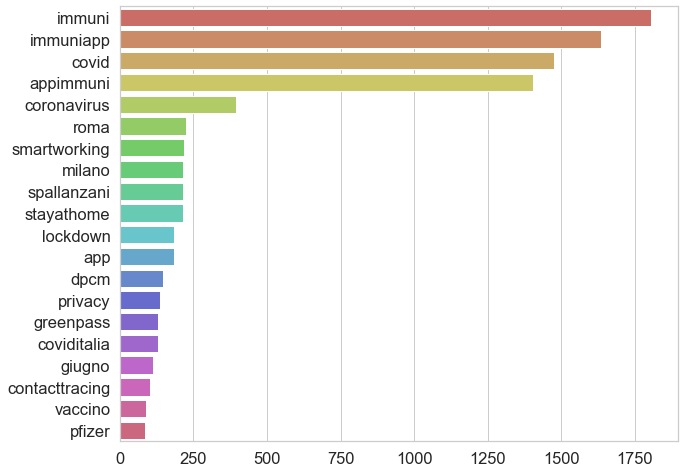
\includegraphics[width = 0.8
    \textwidth]{img/hash_most_freq.jpg}
    \caption{20 hashtag più utilizzati dagli utenti per discutere del tema App Immuni}
    \label{fig:hasht_tweet}
\end{figure}

Il grafico in figura \ref{fig:hasht_tweet}, mostra i dieci hashtag più utilizzati all'interno dei tweet, i quali sono per maggior parte correlati al tema App Immuni e, in generale al Coronavirus, con termini come (\textit{\#covid, \#coronavirus \#smartworking \#lockdown \#dpcm}\footnote{Decreto del Presidente del Consiglio dei ministri, atto amministrativo provvisorio avente forza di legge emanato dal Presiedente del Consiglio sotto la propria responsabilità in casi straordinari di emergenza o necessità}). Oltre a questi hashtag compaiono anche due nomi di città, Roma e Milano, molto importanti soprattutto per i loro ospedali che fin dall'inizio della pandemia si sono impegnate nella ricerca di cure.


Così come si osservava nel grafico \ref{fig:most_common_20_tok}, il termine privacy, oltre ad essere un termine molto utilizzato nei tweet è anche uno degli hashtag utilizzati maggiormente, comparendo in 136 tweet, dimostrando come il tema della privacy abbia acceso il dibatttito diventando uno dei macrotemi di Immuni
Oltre a questo hashtag, un altro molto utilizzato è \textit{\#GreenPass} che compare in 129 tweet scritti nel 2021, un aspetto che conferma ciò che si era osservato nel grafico in figura\ref{fig:tweet_mesi}, in cui nell'agosto 2021 si era osservato un leggero aumento dei tweet dovuti all'integrazione del Green Pass all'interno di Immuni e l'obbligo vaccinale, un tema molto dibattuto e delicato che ha spesso accesso molte discussioni e polarizzato gli utenti. Per questo motivo in alcuni tweet in cui si discute dell'App Immuni vengono quindi utilizzati hashtag come \#\textit{vaccino} e \#\textit{pzfer} che compaiono in circa 80 tweet.


Analizzando invece le caratteristiche linguistiche interne agli hashtag e, in particolare, la lunghezza interna degli hashtag, ossia quante sono le parole che li compongono, si nota come la maggior parte di essi sono molto breve e in media essi sono composti da 6 lettere, un dato che non sorprende vista la brevità dei tweet in termini di caratteri e il fatto che gli hashtag più utilizzati come \#immuni e \#Covid19 hanno quella lunghezza lessicale (Figura \ref{fig: lungh_media_hash_tweet})  
\begin{figure}[H]
    \centering
    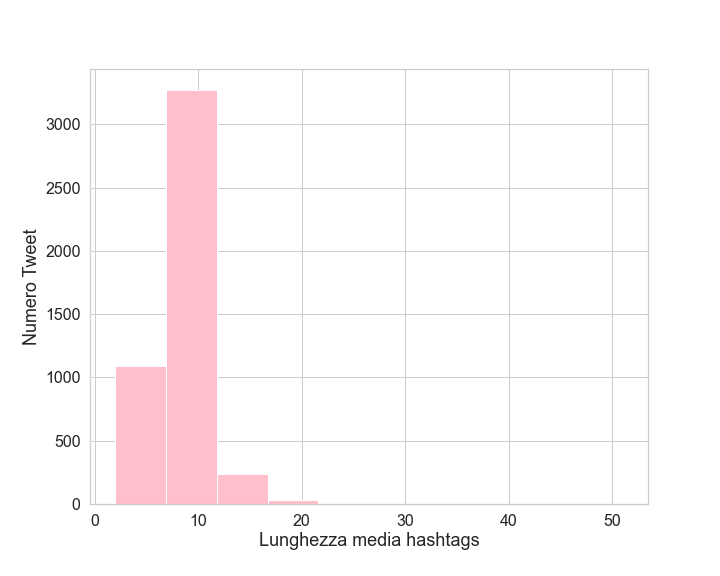
\includegraphics[width=.6
    \textwidth]{img/lunghezza_media_hasht_tweet.png}
    \caption{Quantità media degli hashtag contenuti in ciascun tweet e lunghezza media dei hashtag}
    \label{fig: lungh_media_hash_tweet}
\end{figure}

\section{Distribuzione di \textit{unigrammi}, \textit{bigrammi} e \textit{trigrammi}}
In ultima analisi si è scelto di analizzare la distribuzione delle parole più utilizzate dagli utenti e le combinazioni di parole più frequenti per discutere del tema in analisi.

Per quanto riguarda le singole parole, ossia gli unigrammi (figura \ref{unigrammi}), anche in questo caso abbiamo ottenuto risultati simili a quelli visti precedentemente. Infatti, come si può vedere dalle figure le quali rappresentano rispettivamente la distribuzione degli unigrammi, le parole più utilizzate riguardano il tema appImmuni.

Nel caso invece dei bigrammi (figura \ref{bigrammi}), combinazioni di due parole e dei trigrammi (Figura \ref{trigrammi}), combinazione di tre parole, più frequenti oltre al tema App Immuni, vengono utilizzate fa loro coppie e insiemi di parole rappresentativi della pandemia come \textit{Smartworking} e \textit{Spallanzani}, ossia uno degli ospedali più importanti e impegnati nella ricerca di cure contro il virus 
\begin{figure}[H]
	\centering
	\subfloat[]{
		\label{unigrammi}
		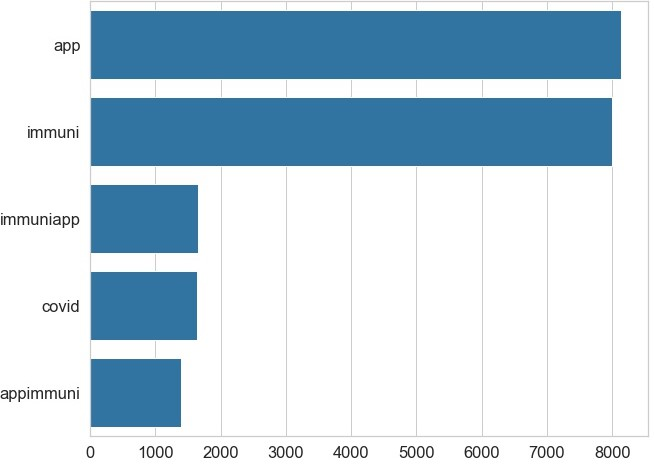
\includegraphics[width=.45\textwidth]{img/unigrammi_df_finale.jpg}
	}
	\quad
	\subfloat[]
	{
		\label{bigrammi}
		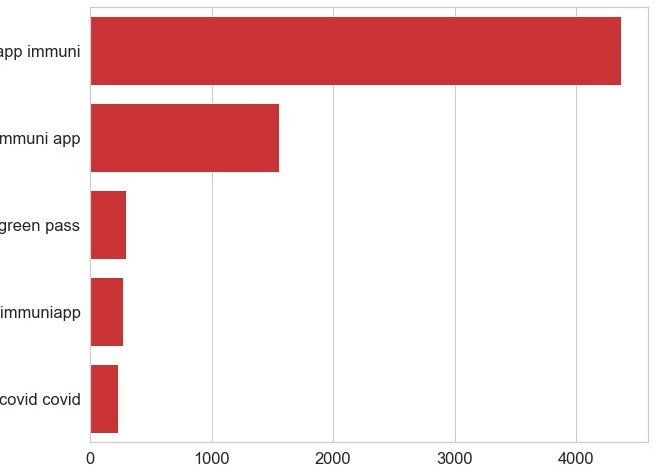
\includegraphics[width=.45\textwidth]{img/bigrammi_df_finale.jpg}
	}    
	\quad
	\subfloat[]
	{
		\label{trigrammi}
		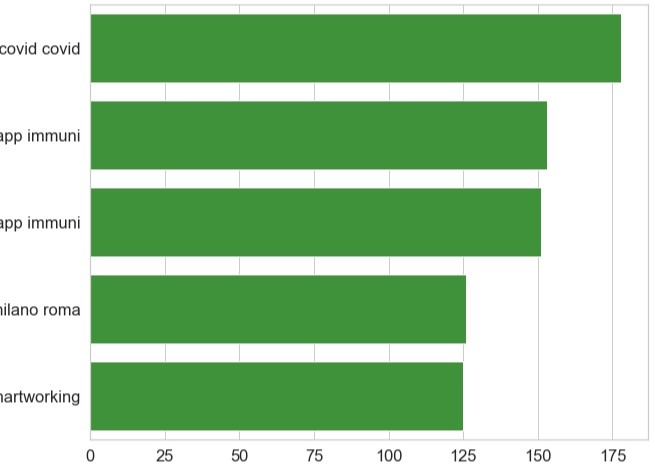
\includegraphics[width=.45\textwidth]{img/trigrammi_df_finale.jpg}
	}    
	\setlength{\belowcaptionskip}{-10pt}
	\caption{Distribuzione dei 5 unigrammi, bigrammi e trigrammi più frequenti utilizzati nella scrittura dei tweet}
	\label{fig: ngrams}
\end{figure}

